\chapter{\textcolor{azulescom}{Diseño}}

\section{Arquitectura del Sistema}

Para el desarrollo del sistema que permitirá a los distintos actores del sector
inmobiliario realizar estimaciones de precios de departamentos en la Ciudad de
México, se propone un sistema web basado en inteligencia artificial usando redes
neuronales que permita a los usuarios ingresar la información del departamento
y obtener una estimación del precio del mismo.

Para el desarrollo del proyecto se utilizará una arquitectura básica de
aplicación web. Siendo así sus elementos un cliente web escrito en React,
una API HTTP con el modelo pre-entrenado en el conjunto de datos extraído, y
configuraciones propias del entorno web para proveer de una buena experiencia
y eficiencia en el uso de la aplicación. En la Figura \ref{fig:arquitectura}
se muestra la arquitectura del sistema.

\begin{figure}[H]
    \centering
    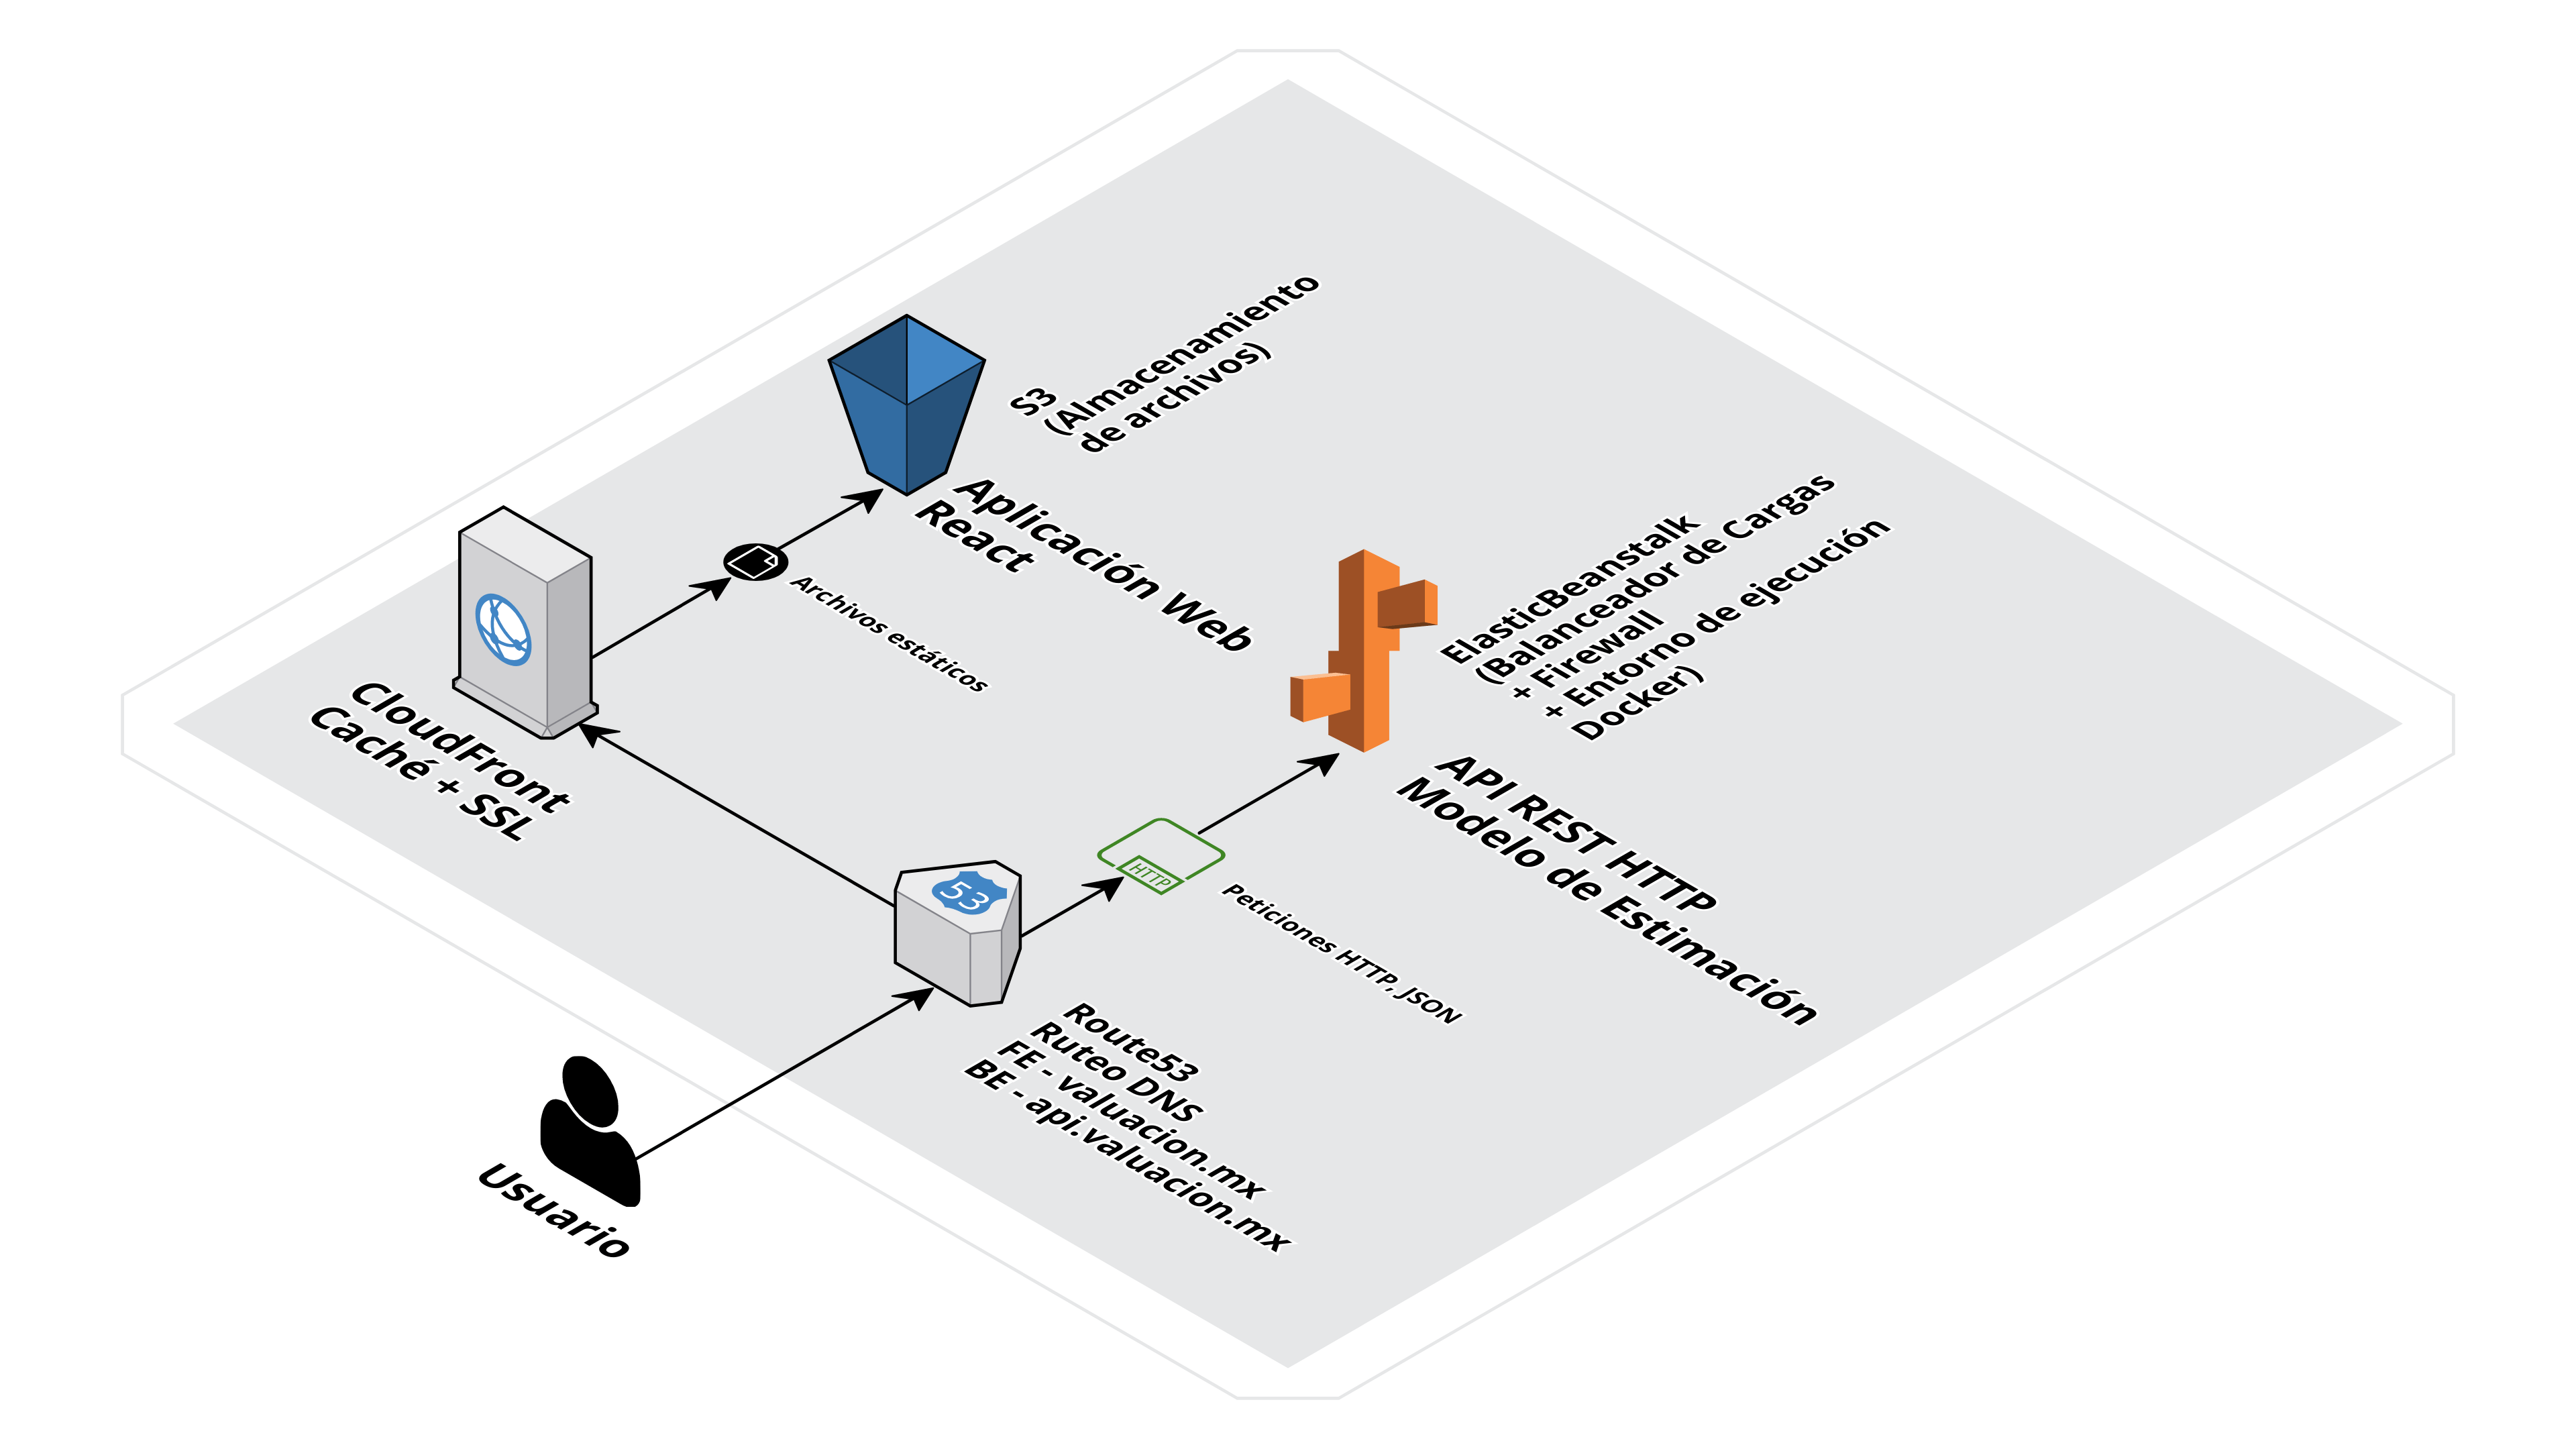
\includegraphics[width=\textwidth]{imagenes/04-diseno/arquitectura-general.png}
    \caption{Arquitectura del sistema}
    \label{fig:arquitectura}
\end{figure}

\subsection{Descripción de la arquitectura}

A continuación se describe cada uno de los elementos que componen la
arquitectura del sistema.

\begin{enumerate}
  \item \textbf{Cliente web}: El cliente web es la interfaz de usuario que
  utilizarán los usuarios para interactuar con el sistema. El cliente web
  está escrito en React, un framework de JavaScript para el desarrollo de
  interfaces de usuario.
  \item \textbf{API REST HTTP}: La API HTTP es el servicio web que provee el
  modelo de inteligencia artificial para la estimación de precios de
  departamentos. La API HTTP está escrita en Python utilizando el framework
  Flask e implementa el modelo de inteligencia artificial utilizando la
  librería TensorFlow.
  \item \textbf{Route53}: Route53 es un servicio de Amazon Web Services que
  permite la administración de los nombres de dominio y la resolución de
  DNS, aquí direccionaremos el dominio de la aplicación web y de la API HTTP.
  \item \textbf{CloudFront}: CloudFront es un servicio de Amazon Web Services
  que permite la distribución de contenido de manera eficiente y segura,
  aquí se almacenarán los archivos estáticos del cliente web. Además, provee
  de un certificado SSL para la comunicación segura entre el cliente web y
  la API HTTP.
  \item \textbf{S3}: S3 es un servicio de Amazon Web Services que permite el
  almacenamiento de archivos de manera segura y escalable, aquí se guardarán
  los archivos estáticos del cliente web.
  \item \textbf{Elastic Beanstalk}: Elastic Beanstalk es un servicio de Amazon
  Web Services que permite el despliegue de aplicaciones web de manera
  rápida y sencilla, aquí se desplegará la API HTTP. Además, provee de un
  certificado SSL para la comunicación segura entre el cliente web y la API
  HTTP.
\end{enumerate}

\subsection{Caso de Uso}

Un caso de uso se define como \textit{una secuencia de acciones, incluyendo variaciones,
que el sistema puede ejecutar y que produce un resultado observable de valor
para un actor que interactúa con el sistema} \cite{jacobson2021unified}.

Dado que el proyecto se compone de una única interacción entre el usuario y
el sistema, se cuenta con un único caso de uso, dónde el usuario envía la
información pertinente al sistema y este le devuelve la estimación de precio
para el departamento. En la Figura \ref{fig:caso_de_uso} se muestra el diagrama
de caso de uso.

\begin{figure}[H]
    \centering
    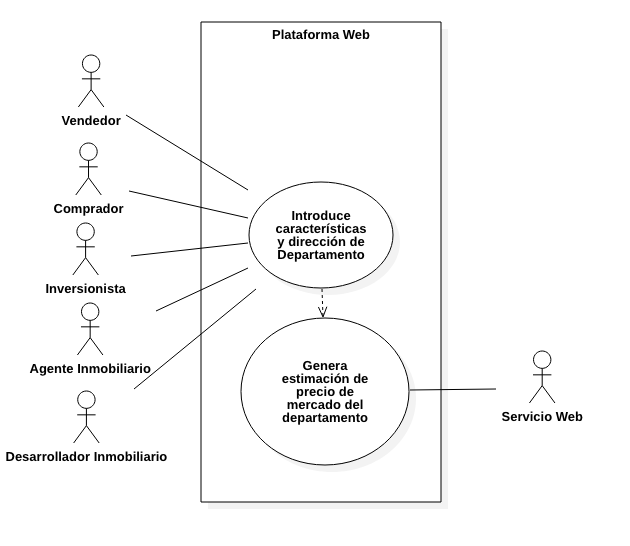
\includegraphics[width=0.8\textwidth]{imagenes/04-diseno/caso-de-uso.png}
    \caption{Diagrama de caso de uso}
    \label{fig:caso_de_uso}
\end{figure}

En el Cuadro \ref{tab:caso_de_uso} se muestra la descripción del caso de uso.

\begin{table}[H]
    \centering
    \begin{tabular}{|c|p{0.7\textwidth}|}
        \hline
        \textbf{Caso de Uso} & Estimar precio de un departamento \\
        \hline
        \textbf{Descripción} & El usuario envía la información del
        departamento al sistema y este le devuelve la estimación de precio. \\
        \hline
        \textbf{Actores} & Usuario \\
        \hline
        \textbf{Precondiciones} & El usuario debe tener la información del
        departamento. \\
        \hline
        \textbf{Postcondiciones} & El usuario recibe la estimación de precio
        del departamento. \\
        \hline
        \textbf{Escenario Principal} & \begin{enumerate}
            \item El usuario envía la información del departamento al sistema.
            \item El sistema devuelve la estimación de precio del departamento.
        \end{enumerate} \\
        \hline
    \end{tabular}
    \caption{Descripción del caso de uso}
    \label{tab:caso_de_uso}
\end{table}

\subsection{Reglas de Negocio}

Las reglas de negocio permiten definir las condiciones para establecer un negocio o
precisar de qué forma se controlará el comportamiento de los eventos dentro de
este. Muy importante resulta establecer los pasos que se deben seguir para alcanzar las
metas y objetivos del mismo. Las reglas de negocio son requisitos que definen cómo el
negocio debe operar \cite{181439409006}.

A continuación se presentan las reglas de negocio del sistema:

\begin{enumerate}
  \item \textbf{Validez de la Dirección:} Cada dirección ingresada debe ser
    verificada contra una base de datos actualizada de direcciones válidas de la
    Ciudad de México para asegurar la precisión de la ubicación y la relevancia
    de la estimación de precios proporcionada.
  \item \textbf{Integridad de los Datos:} Los usuarios deben proporcionar información
    completa y precisa para cada departamento. El sistema rechazará entradas que
    contengan datos faltantes, ambiguos o claramente erróneos, como valores
    negativos para áreas de superficie.
  \item \textbf{Privacidad de los Datos:} La plataforma se compromete a proteger
    la privacidad de los usuarios. Los datos personales recopilados durante el
    proceso de estimación se manejarán de acuerdo con las normativas de protección
    de datos vigentes, asegurando la confidencialidad y el derecho a la privacidad
    de los usuarios.
  \item \textbf{Limitaciones de la Estimación:} Las estimaciones generadas son
    aproximaciones basadas en modelos matemáticos y no pueden capturar todas las
    variables únicas de cada propiedad. Se debe comunicar claramente a los
    usuarios que el precio de mercado real puede variar.
  \item \textbf{Actualización de Datos:} Para mantener la precisión de las
    estimaciones, el modelo subyacente se recalibrará periódicamente incorporando
    nuevos datos del mercado, reflejando así los cambios y tendencias actuales en
    los precios de los departamentos.
  \item \textbf{Tratamiento de Outliers:} Durante la fase de análisis y antes
    del entrenamiento del modelo predictivo, se identificarán y excluirán los
    valores atípicos para evitar distorsiones en la estimación de precios.
  \item \textbf{Selección de Características:} El modelo se construirá utilizando
    únicamente aquellas características que tengan una correlación estadísticamente
    significativa con el precio del departamento, optimizando así la precisión de
    las predicciones.
  \item \textbf{Manejo de ``En Construcción'':} Los departamentos en fase de construcción
    se manejarán con una etiqueta especial dentro del sistema. Se asignará un valor
    de antigüedad convencional o se desarrollará un tratamiento estadístico
    alternativo para estos casos.
  \item \textbf{Acceso al Servicio:} La plataforma implementará políticas de uso
    justo para garantizar la disponibilidad y la fiabilidad del servicio, evitando
    la sobrecarga del sistema y asegurando un acceso equitativo para todos los usuarios.
  \item \textbf{Respuesta del Sistema:} El sistema está diseñado para proporcionar
    una estimación de precios de manera eficiente y dentro de un marco de tiempo
    razonable, buscando maximizar la experiencia del usuario y la utilidad del
    servicio.
\end{enumerate}

\subsection{Historias de Usuario}

Una historia de usuario describe alguna funcionalidad que debe ser valiosa a un
usuario o comprador de un sistema o software \cite{cohn2004user}. Las historias de usuario se
componen de tres aspectos fundamentales:

\begin{enumerate}
  \item \textbf{Descripción:} Una descripción corta de la historia de usuario.
  \item \textbf{Criterios de Aceptación:} Una lista de criterios que deben ser
    cumplidos para que la historia de usuario sea aceptada.
  \item \textbf{Conversaciones:} Una lista de conversaciones que se han tenido
    con el usuario para entender mejor la historia de usuario.
\end{enumerate}

Al igual que en la sección anterior, dado que el
proyecto se compone de una única interacción entre el usuario y el sistema,
se cuenta con una única historia de usuario, dónde el usuario envía la
información pertinente al sistema y este le devuelve la estimación de precio
para el departamento.  En el Cuadro \ref{tab:historias_de_usuario} se
muestran las historias de usuario del sistema.

\begin{table}[H]
    \centering
    \begin{tabular}{|c|p{0.7\textwidth}|}
        \hline
        \textbf{Historia de Usuario} & Estimar precio de un departamento \\
        \hline
        \textbf{Descripción} & El usuario envía la información del
        departamento al sistema y este le devuelve la estimación de precio. \\
        \hline
        \textbf{Criterios de Aceptación} & \begin{enumerate}
            \item El usuario debe tener la información del departamento.
            \item El usuario debe recibir la estimación de precio del
            departamento.
        \end{enumerate} \\
        \hline
    \end{tabular}
    \caption{Historia de usuario}
    \label{tab:historias_de_usuario}
\end{table}

\subsection{Diagrama de Secuencia}

Los diagramas de secuencia se utilizan para presentar el comportamiento dinámico
del diseño de un sistema, mientras que los diagramas de clases representan la
estructura estática del sistema. Como uno de los dos tipos de diagramas de
interacción UML, un diagrama de secuencia muestra las interacciones entre
objetos organizados en una secuencia temporal \cite{1290469}.

En la Figura \ref{fig:diagrama_de_secuencia} se muestra el diagrama de
secuencia correspondiente a la interacción entre el usuario y el sistema.

\begin{figure}[H]
    \centering
    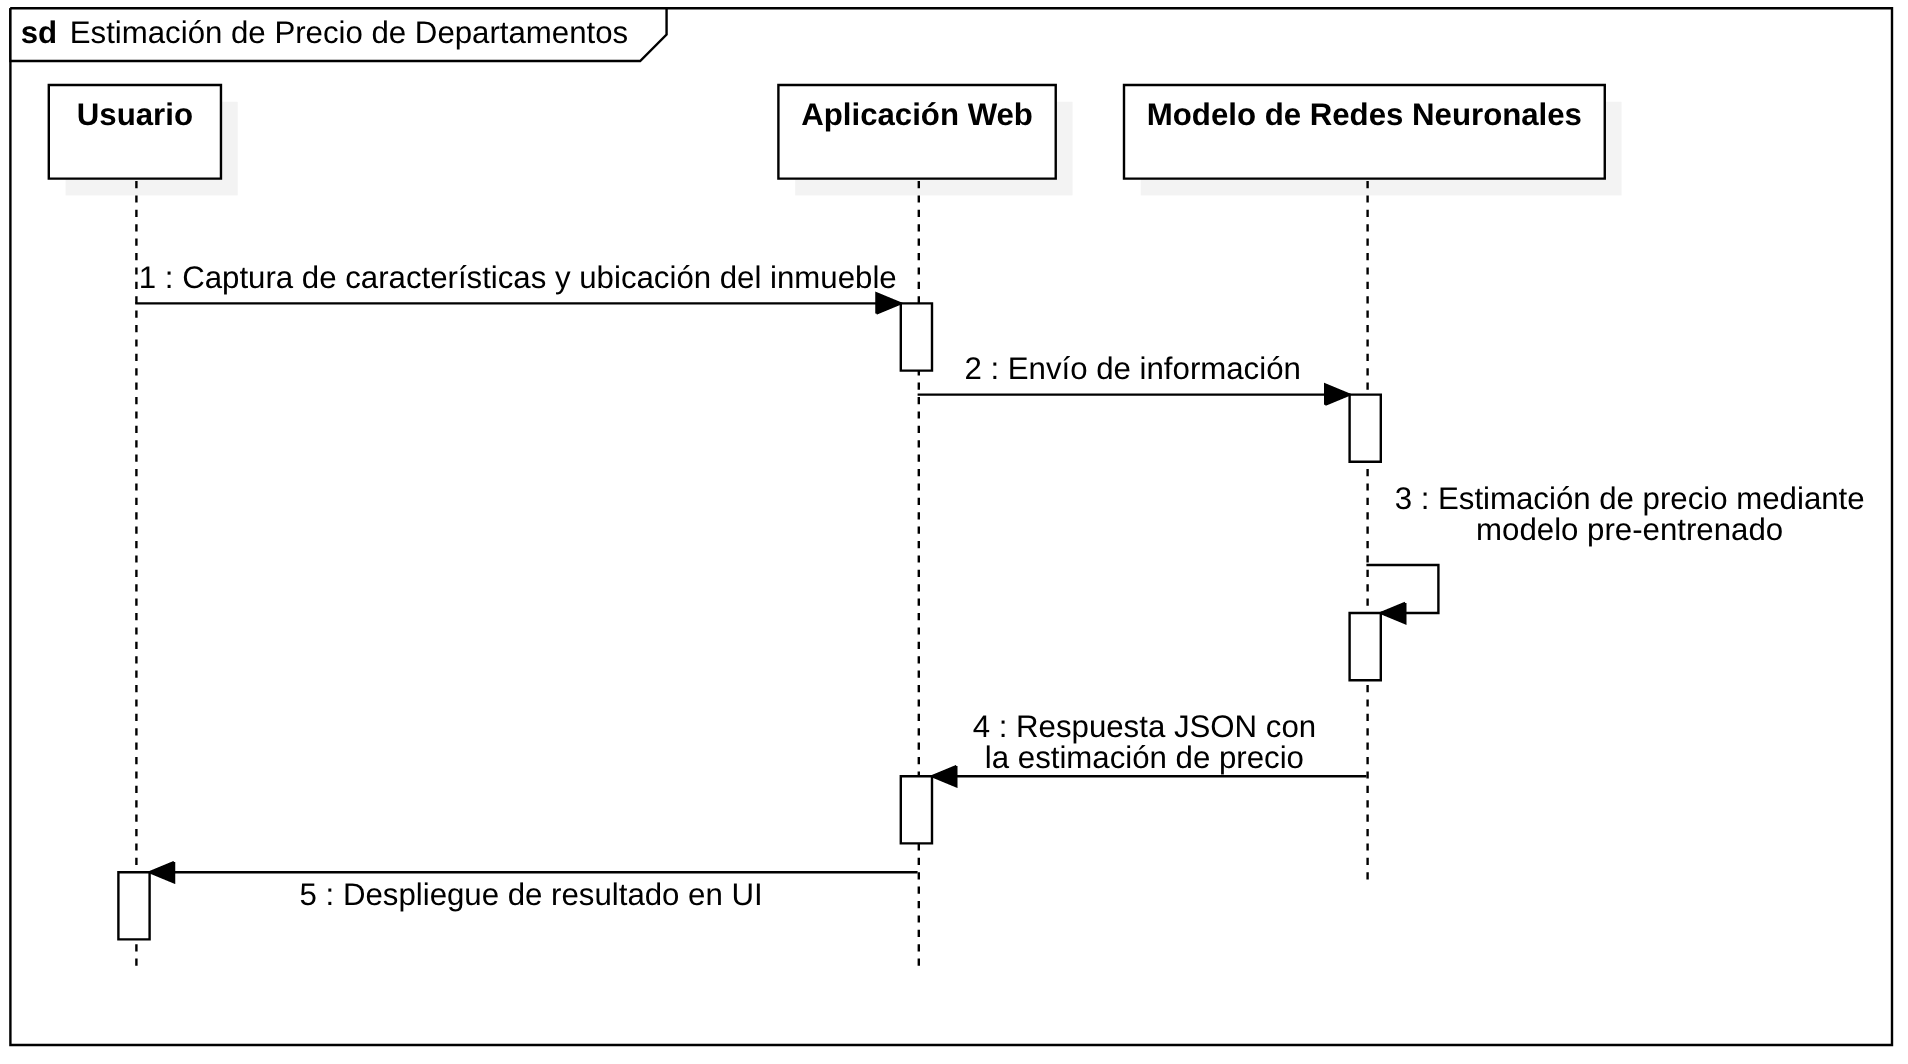
\includegraphics[width=0.8\textwidth]{imagenes/04-diseno/secuencia.png}
    \caption{Diagrama de secuencia}
    \label{fig:diagrama_de_secuencia}
\end{figure}

\subsection{Requerimientos Funcionales}

Los requerimientos funcionales se refieren a las funcionalidades que el
sistema debe proveer al usuario \cite{geeksforgeeks2023functional}. A
continuación se presenta un listado con los requerimientos funcionales del
sistema. Aunque.

\begin{enumerate}
    \item \textbf{Ingreso de información del departamento}: Permitir al usuario
    ingresar detalles de un departamento (ubicación, superficie, cantidad de
    dormitorios, cantidad de baños, antigüedad, etc.).
    \item \textbf{Estimación de precio del departamento}: Permitir al usuario
    obtener una estimación del precio del departamento ingresado.
    \item \textbf{Visualización de información del departamento}: Permitir al
    usuario visualizar la información ingresada del departamento.
    \item \textbf{Interfaz de usuario intuitiva}: La interfaz de usuario debe
    ser intuitiva y fácil de usar.
\end{enumerate}

\subsection{Requerimientos No Funcionales}

Los requerimientos no funcionales sirven para especificar los criterios que
se deben cumplir para que el sistema sea aceptado por el usuario
\cite{geeksforgeeks2023functional}. A continuación se presenta un listado
con los requerimientos no funcionales del sistema.

\begin{enumerate}
    \item \textbf{Tiempo de respuesta}: El sistema debe responder en un tiempo
    menor a 1 segundo.
    \item \textbf{Precisión}: El sistema debe tener una precisión mayor al 80\%.
    \item \textbf{Usabilidad}: El sistema debe ser fácil de usar.
    \item \textbf{Escalabilidad}: El sistema debe ser escalable.
    \item \textbf{Disponibilidad}: El sistema debe estar disponible las 24
    horas del día.
    \item \textbf{Seguridad}: El sistema debe ser seguro.
\end{enumerate}

\section{Conjunto de Datos}

En este apartado se abordará el conjunto de datos utilizado para el desarrollo
del proyecto. Se explicará la descripción del conjunto de datos, la obtención
del conjunto de datos y el preprocesamiento del conjunto de datos.

\subsection{Descripción del Conjunto de Datos}

Dado que el proyecto se basa en la estimación de precios de departamentos en
la Ciudad de México, se utilizó un conjunto de datos de departamentos con
características como ubicación, superficie, cantidad de dormitorios, cantidad
de baños, antigüedad, etc. y su precio. El conjunto de datos fue obtenido de
distintas fuentes, como por ejemplo, el portal de bienes raíces inmuebles24.com
\cite{inmuebles24url}.

El conjunto de datos cuenta con 40,000 registros, de los cuales 18,000 son únicos.
Debido a que los portales inmobiliarios pueden o no incluir múltiples otros
datos como el número de estacionamientos, el número de pisos, etc., se decidió
utilizar únicamente los datos que se encuentran en la mayoría de los registros,
es decir, los datos que se encuentran en más del 50\% de los registros. En la
Tabla \ref{tab:datos} se muestran los datos que se utilizaron para el desarrollo
del proyecto.

\begin{table}[H]
    \centering
    \begin{tabular}{|p{0.25\textwidth}|p{0.7\textwidth}|}
        \hline
        \rowcolor{azulclaro}
        \centering\textbf{Datos} & \centering\textbf{Descripción}\arraybackslash \\
        \hline
        \textbf{Ubicación} & Alcaldía, colonia, latitud y longitud. \\
        \hline
        \textbf{Superficie} & Superficie total y superficie construida. \\
        \hline
        \textbf{Dormitorios} & Cantidad de dormitorios. \\
        \hline
        \textbf{Baños} & Cantidad de baños. \\
        \hline
        \textbf{Antigüedad} & Antigüedad del departamento. \\
        \hline
        \textbf{Precio} & Precio del departamento. \\
        \hline
    \end{tabular}
    \caption{Datos utilizados para el desarrollo del proyecto}
    \label{tab:datos}
\end{table}

Adicional, se retiene el ID original del anuncio, para poder identificar los
registros duplicados y eliminarlos.

\subsection{Obtención del Conjunto de Datos}

Para obtener el conjunto de datos, se construyó un \textit{web scraper} que
extrae la información de los departamentos de la Ciudad de México del portal
Inmuebles24 \cite{inmuebles24url}. El \textit{web scraper} fue desarrollado en
Bash utilizando la herramienta \textit{curl} para realizar las peticiones HTTP
y la herramienta \textit{jq} para procesar los datos en formato JSON.

Dicho \textit{web scraper} se ejecutó durante 7 horas, y los datos obtenidos
se guardaron en un archivo JSON, con un peso aproximado de 800MB. En la Figura
\ref{fig:web_scraper} se muestra el diagrama de flujo del \textit{web scraper}.

\begin{figure}[H]
    \centering
    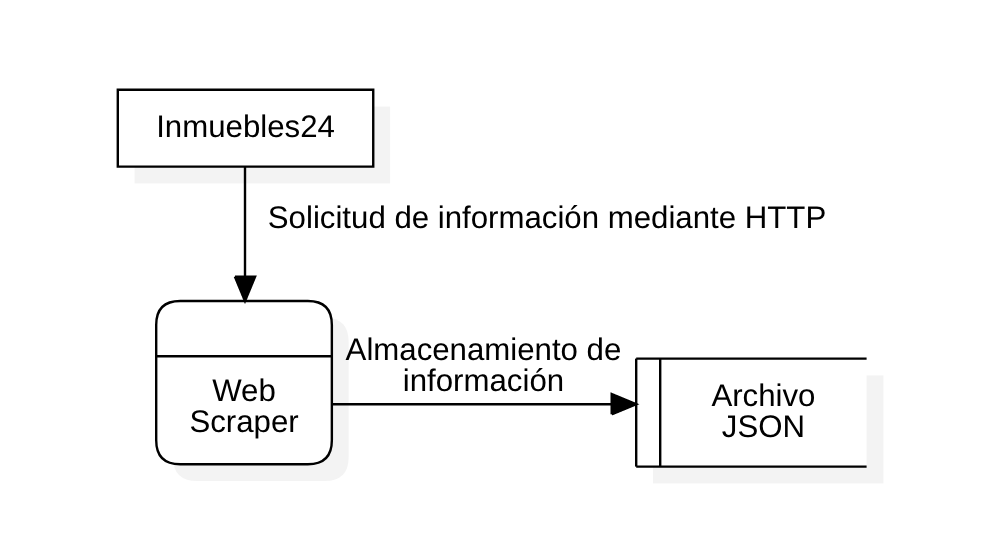
\includegraphics[width=0.8\textwidth]{imagenes/04-diseno/arquitectura-web-scraper.png}
    \caption{Diagrama de flujo del \textit{web scraper}}
    \label{fig:web_scraper}
\end{figure}

En el listado \ref{lst:web_scraper} se muestra el código fuente del \textit{web
scraper}.

\begin{lstlisting}[language=bash, caption={Código fuente del \textit{web scraper}}, label={lst:web_scraper}]
#!/bin/bash
# Este es un pequeño script de bash que usa cURL para simular correctamente a
# el ambiente del navegador para hacer una petición al API de Inmuebles24 y
# así poder obtener la lista de departamentos en venta en la Ciudad de México.

# Verificamos que jq esté instalado.
if ! command -v jq &> /dev/null
then
    echo "No se encontró jq, por favor instálalo antes de continuar."
    exit
fi

# Generamos un nombre de archivo único para esta ejecución.
filename=scrape-$(date +"%Y%m%d-%H-%M-%S").json

# Inicializamos un arreglo JSON vacío en el archivo.
echo "[" > "$filename"

# Página inicial.
pagina=1

# Ciclo para recorrer los primeros 2015 resultados.
# (Nota: el valor se deberá cambiar manualmente dependiendo de los anuncios
#        disponibles en la plataforma)
while (( pagina <= 2015)); do
  # Imprimos en qué página vamos.
  echo "Obteniendo página #$pagina..."

  # Realizamos el request a inmuebles24.com
  response=$(curl -s 'https://www.inmuebles24.com/rplis-api/postings' \
    -H 'authority: www.inmuebles24.com' \
    -H 'accept: */*' \
    -H 'accept-language: en' \
    -H 'content-type: application/json' \
    -H 'dnt: 1' \
    -H 'origin: https://www.inmuebles24.com' \
    -H 'referer: https://www.inmuebles24.com/departamentos-en-venta-en-ciudad-de-mexico.html' \
    -H 'sec-ch-ua: "Chromium";v="118", "Google Chrome";v="118", "Not=A?Brand";v="99"' \
    -H 'sec-ch-ua-mobile: ?0' \
    -H 'sec-ch-ua-platform: "macOS"' \
    -H 'sec-fetch-dest: empty' \
    -H 'sec-fetch-mode: cors' \
    -H 'sec-fetch-site: same-origin' \
    -H 'user-agent: Mozilla/5.0 (Macintosh; Intel Mac OS X 10_15_7) AppleWebKit/537.36 (KHTML, like Gecko) Chrome/118.0.0.0 Safari/537.36' \
    -H 'x-requested-with: XMLHttpRequest' \
    --data-raw '{"q":null,"direccion":null,"moneda":null,"preciomin":null,"preciomax":null,"services":"","general":"","searchbykeyword":"","amenidades":"","caracteristicasprop":null,"comodidades":"","disposicion":null,"roomType":"","outside":"","areaPrivativa":"","areaComun":"","multipleRets":"","tipoDePropiedad":"2","subtipoDePropiedad":null,"tipoDeOperacion":"1","garages":null,"antiguedad":null,"expensasminimo":null,"expensasmaximo":null,"habitacionesminimo":0,"habitacionesmaximo":0,"ambientesminimo":0,"ambientesmaximo":0,"banos":null,"superficieCubierta":1,"idunidaddemedida":1,"metroscuadradomin":null,"metroscuadradomax":null,"tipoAnunciante":"ALL","grupoTipoDeMultimedia":"","publicacion":null,"sort":"more_recent","etapaDeDesarrollo":"","auctions":null,"polygonApplied":null,"idInmobiliaria":null,"excludePostingContacted":"","banks":"","places":"","condominio":"","pagina":'"$pagina"',"city":null,"province":"69","zone":null,"valueZone":null,"subZone":null,"coordenates":null}' \
    --compressed)

  # Obtenemos el arreglo de anuncios de la respuesta.
  list_postings=$(echo "$response" | jq '.listPostings')

  # Imprimimos la cantidad de anuncios en la página.
  echo "Cantidad de anuncios: $(echo "$list_postings" | jq '. | length')"

  # Obtenemos el arreglo de anuncios de la respuesta y removemos los corchetes iniciales y finales.
  list_postings2=${list_postings:1:${#list_postings}-2}

  # Agregamos los datos de list_postings al archivo, seguido de una coma para separarlo del siguiente set de datos,
  # solo si hay datos para agregar.
  if [[ -n $list_postings2 ]]; then
    echo "$list_postings2," >>"$filename"
  fi

  # Incrementar el número de página para la siguiente iteración
  ((pagina++))
done

# Cuando terminamos de iterar, removemos la última coma y agregamos un corchete final.
sed -i '' -e '$ s/,$//g' -e '$ s/$/]/' "$filename"

# Imprimimos el nombre del archivo donde se guardaron los datos.
echo "Datos guardados en: $filename"
\end{lstlisting}

\subsection{Preprocesamiento del Conjunto de Datos}

Debido a que los datos obtenidos son súmamente extensos (cada anuncio puede
incluir inclusive información personal del anunciante como nombre, teléfono,) y
suponen riesgos de privacidad, se optó por la construcción de un \textit{Convertidor}
el cual se encarga de procesar el archivo JSON obtenido por el \textit{web scraper}
y generar un nuevo archivo CSV con los datos que se utilizarán para el desarrollo
del proyecto.

En la Figura \ref{fig:arquitectura-conversor} se muestra el diagrama de flujo del
\textit{Convertidor} propuesto.

\begin{figure}[H]
    \centering
    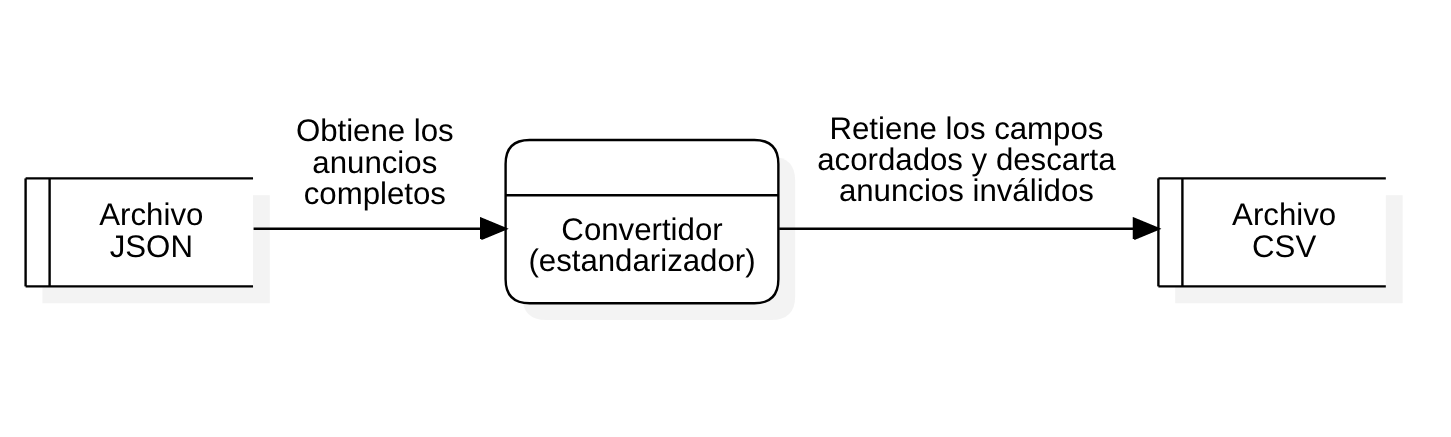
\includegraphics[width=0.8\textwidth]{imagenes/04-diseno/arquitectura-convertidor.png}
    \caption{Diagrama de flujo del \textit{Convertidor}}
    \label{fig:arquitectura-conversor}
\end{figure}

\section{Limpieza del Conjunto de Datos}

Tal y cómo se mostró en la sección del análisis exploratorio econométrico, el
dataset final que se utilizará para el entrenamiento del modelo de estimación
de precios estará sujeto a una serie de transformaciones y limpiezas que
permitirán obtener un dataset más limpio y con mejores características para
el entrenamiento del modelo. En esta sección se explicarán las transformaciones
y limpiezas que se realizarán al dataset.

\subsection{Detección de Outliers}

Para la detección de outliers se utilizará el método de los cuartiles, el cual
consiste en calcular el rango intercuartil (IQR) y luego multiplicarlo por 1.5.
Los valores que se encuentren por encima de este valor serán considerados
outliers.

\subsection{Detección de Valores Faltantes}

Para la detección de valores faltantes se utilizará el método de la imputación
por la media, el cual consiste en reemplazar los valores faltantes por la media
de los valores de la columna correspondiente.

\subsection{Detección de Valores Atípicos}

Para la detección de valores atípicos se utilizará el método de la imputación
por la mediana, el cual consiste en reemplazar los valores atípicos por la
mediana de los valores de la columna correspondiente.

\subsection{Detección de Valores Negativos}

Para la detección de valores negativos se utilizará el método de la imputación
por la mediana, el cual consiste en reemplazar los valores negativos por la
mediana de los valores de la columna correspondiente.

\subsection{Detección de Valores Categóricos}

Para la detección de valores categóricos se utilizará el método de la
codificación one-hot, el cual consiste en crear una columna por cada valor
categórico y asignar un 1 si el valor categórico está presente en el registro
y un 0 si no lo está.

\subsection{Detección de Valores Numéricos}

Para la detección de valores numéricos se utilizará el método de la
normalización, el cual consiste en normalizar los valores numéricos para que
estén en el conjunto de números reales.


\section{Modelo de Estimación de Precios}

En esta sección, describiremos el diseño e implementación de un modelo de
estimación de precios para una plataforma web de valuación inmobiliaria con
Inteligencia Artificial. La estrategia principal consiste en utilizar múltiples
modelos para generar diversas estimaciones de precios, seleccionando posteriormente
la más adecuada. Esta aproximación permite aprovechar las fortalezas de diferentes
técnicas de aprendizaje automático, optimizando así la precisión y fiabilidad de
las estimaciones.

\subsection{Arquitectura del Modelo}

La arquitectura del modelo se compone de tres enfoques principales: redes neuronales,
máquinas de soporte vectorial (SVM) y árboles aleatorios. Cada uno de estos métodos
aporta características únicas en la estimación de precios, permitiendo abarcar
distintos aspectos del problema. En la Figura \ref{fig:arquitectura-modelo} se
muestra la arquitectura del modelo.

\begin{figure}[H]
    \centering
    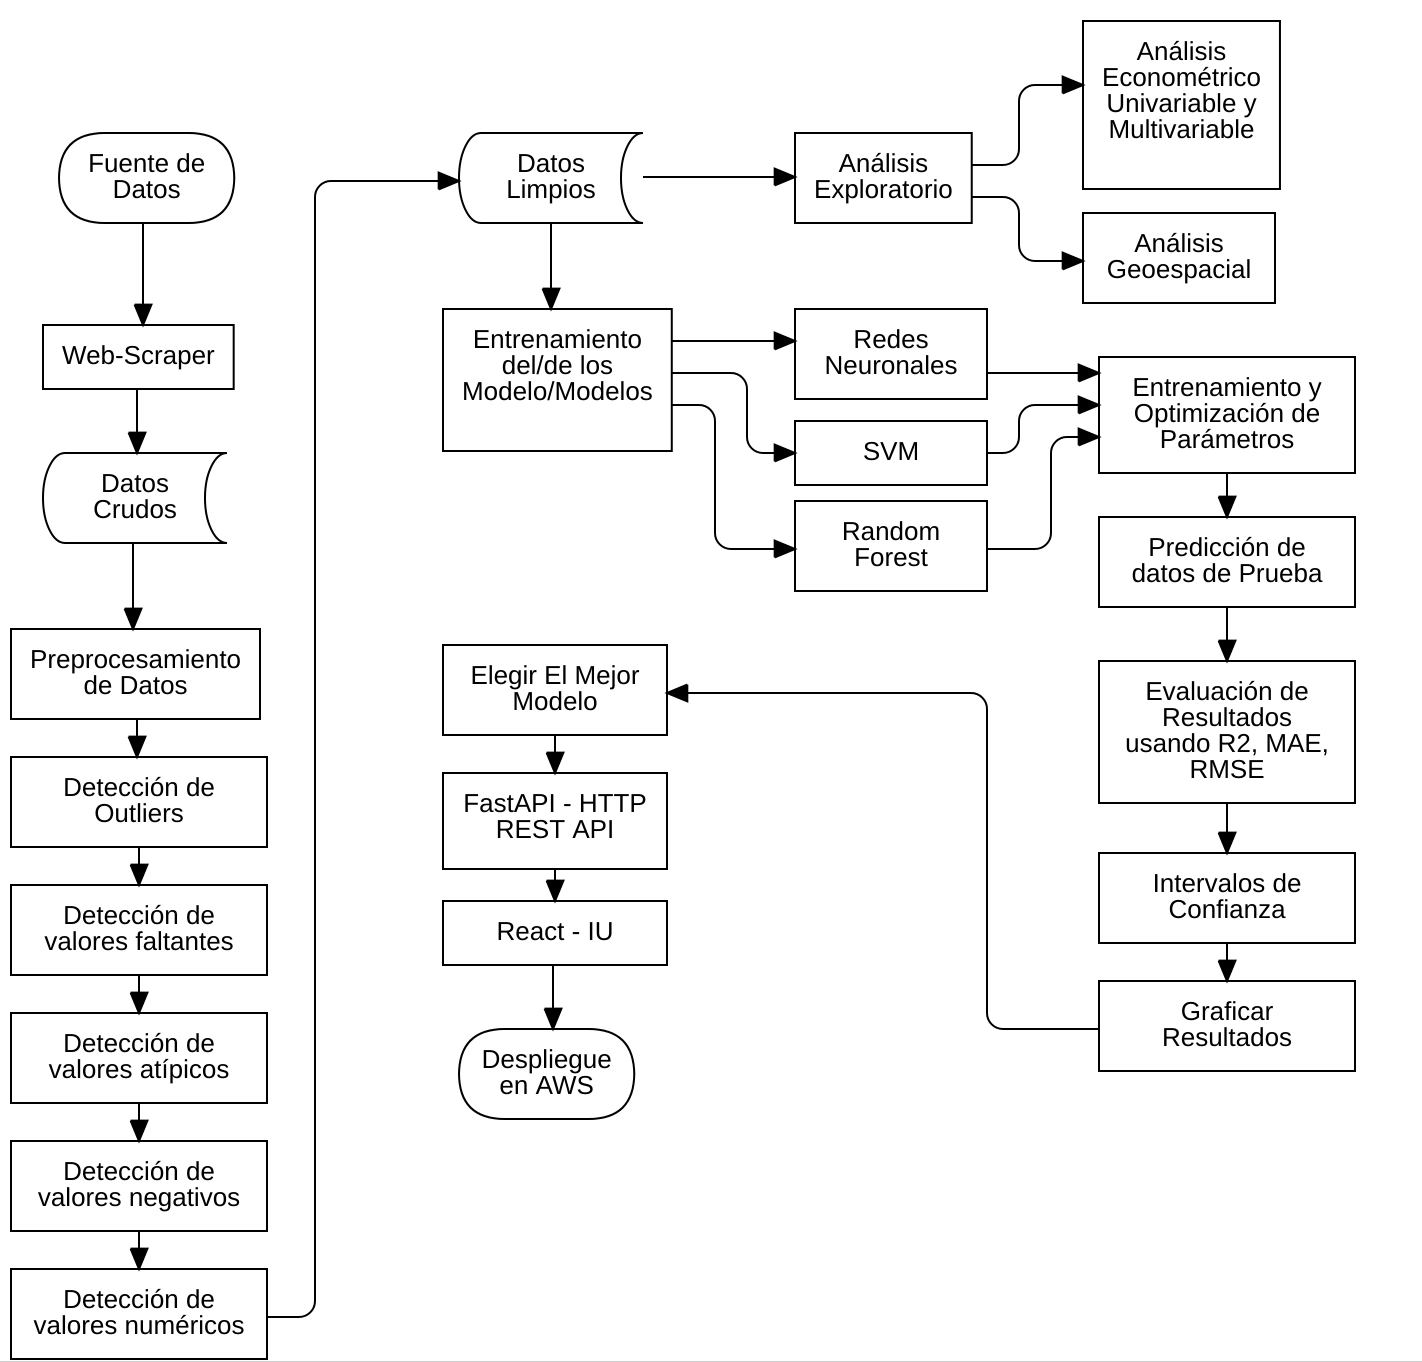
\includegraphics[width=0.8\textwidth]{imagenes/04-diseno/arquitectura-modelo.png}
    \caption{Arquitectura del modelo}
    \label{fig:arquitectura-modelo}
\end{figure}

\subsubsection{Red Neuronal}
Las redes neuronales se utilizarán para captar patrones complejos en los datos. Su
capacidad para aprender representaciones no lineales las hace especialmente útiles
en el contexto de los datos inmobiliarios, que a menudo contienen relaciones
complejas entre las características.

\subsubsection{Máquina de Soporte Vectorial}
Las máquinas de soporte vectorial (SVM) se aplicarán para clasificar y predecir
los precios de los inmuebles. Su eficacia en espacios de alta dimensión y con
margen de separación claro las hace valiosas para este tipo de estimaciones.

\subsubsection{Árboles Aleatorios}
Los árboles aleatorios, o bosques aleatorios, se usarán por su habilidad para
manejar grandes conjuntos de datos y su resistencia a overfitting. Son útiles
para capturar relaciones no lineales sin necesidad de un preprocesamiento extenso
de los datos.

\subsection{Entrenamiento del Modelo}

El entrenamiento de los modelos se realizará utilizando librerías populares en
Python, como Scikit-learn, TensorFlow y PyTorch. Estas herramientas proporcionan
una amplia gama de funcionalidades para manejar distintos aspectos del entrenamiento
de modelos de aprendizaje automático, desde la preprocesamiento de datos hasta la
optimización de hiperparámetros.

\subsection{Evaluación del Modelo}

La evaluación de los modelos implicará el uso de métricas estándar como el error
cuadrático medio (MSE) y el coeficiente de determinación (R²). Estas métricas
permitirán determinar la precisión de las estimaciones de precios y comparar
la efectividad de los diferentes modelos implementados.

\subsection{Despliegue del Modelo}

Finalmente, el despliegue del modelo se llevará a cabo localmente. Los modelos
entrenados se integrarán en un contenedor Docker, junto con un servicio desarrollado
en FastAPI. Esta configuración permitirá realizar consultas al modelo a través de
una API, donde el usuario podrá enviar la ubicación y características del inmueble,
recibiendo a cambio las estimaciones de precios proporcionadas por los distintos
modelos.


\section{Aplicación Web}

El producto final del proyecto es una aplicación web que permita a los usuarios
realizar estimaciones de precios de departamentos en la Ciudad de México. En
esta sección se explicará la arquitectura de la aplicación web, la interfaz de
usuario y el funcionamiento de la aplicación web.

\subsection{Wireframes}

Para el desarrollo de la interfaz de usuario se utilizaron wireframes, los
cuales son una representación visual de la estructura de una página web. En la
Figura \ref{fig:wireframes} se muestra el wireframe inicial de la aplicación
web, es decir, lo que el usuario verá al ingresar a la aplicación web. Consiste
en un formulario con los campos necesarios para ingresar la información del
departamento y un botón para enviar la información al sistema. Se decidió
utilizar un formulario debido a que es la manera más sencilla de ingresar
información en una aplicación web.

\begin{figure}[H]
    \centering
    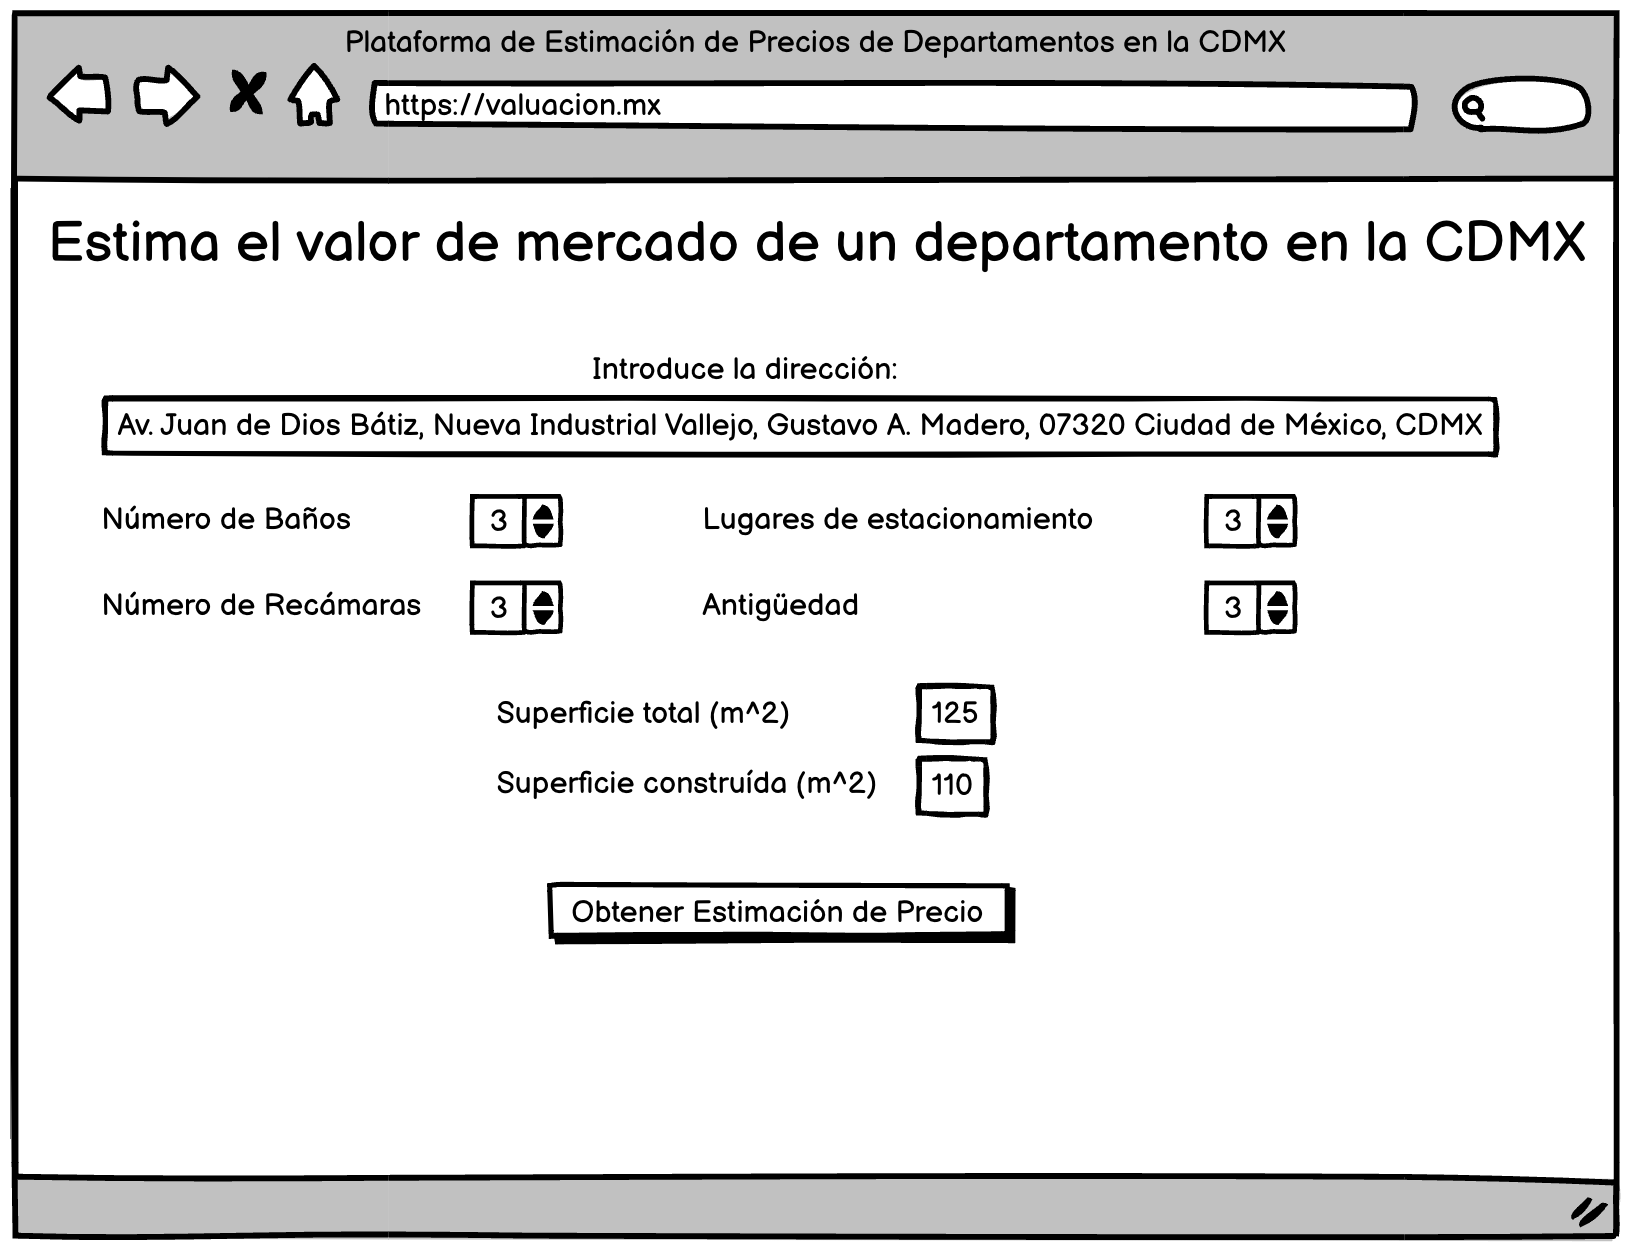
\includegraphics[width=0.8\textwidth]{imagenes/04-diseno/wireframe-1.png}
    \caption{Wireframe con el estado inicial de la aplicación web}
    \label{fig:wireframes}
\end{figure}

Una vez que el usuario haya hecho click en el botón con el cual se envía la
información capturada en el formulario, se mostrará una pantalla de carga,
mientras el sistema procesa la información y devuelve la estimación de precio
del departamento. En la Figura \ref{fig:wireframes-2} se muestra el wireframe
correspondiente al resultado final del sistema, es decir, la estimación de
precio del departamento.

\begin{figure}[H]
    \centering
    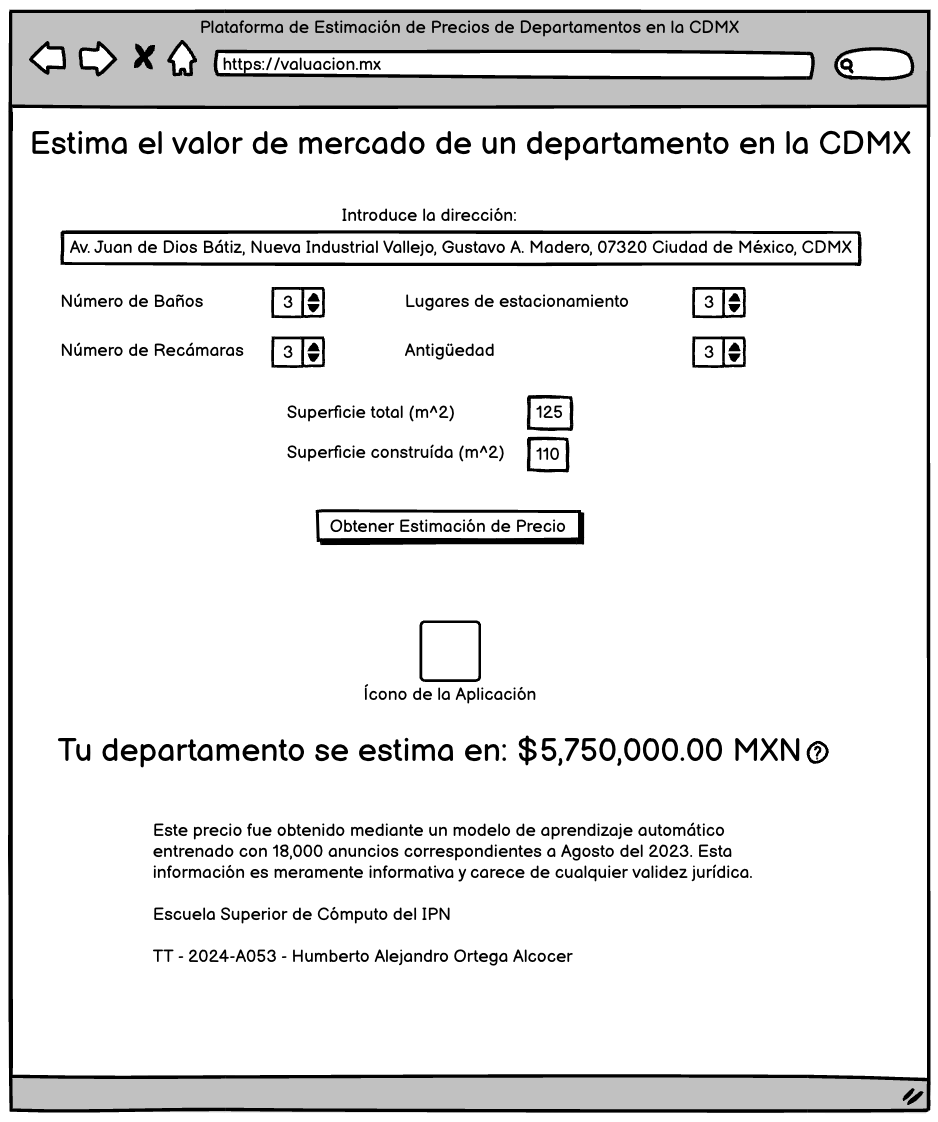
\includegraphics[width=0.8\textwidth]{imagenes/04-diseno/wireframe-2.png}
    \caption{Wireframe con la estimación de precio del departamento}
    \label{fig:wireframes-2}
\end{figure}

\subsection{Dependencias externas}

Debido a que la aplicación web deberá ofrecer una funcionalidad de geo-localización,
es decir, obtener las coordenadas geográficas a partir de una dirección, se requiere
de la integración de un servicio externo que permita realizar dicha funcionalidad.
Esto ya que la implementación de un servicio propio de geo-localización es una tarea
compleja y que requiere de una gran cantidad de recursos. Sobre todo porque
la información geoespacial de la Ciudad de México es muy extensa y compleja, además
de estar sujeta a una constante actualización y modificación.

\subsubsection{Google Maps}

Google Maps es un servicio de Google que permite la visualización de mapas
geográficos. Además, ofrece una API que permite la integración de Google Maps
en aplicaciones web. Dicha API ofrece una funcionalidad de geo-localización,
la cual permite obtener las coordenadas geográficas a partir de una dirección.
En la Figura \ref{fig:google-maps} se muestra un ejemplo de la funcionalidad
de geo-localización de Google Maps \cite{google_geocoding_2023}.

\begin{figure}[H]
    \centering
    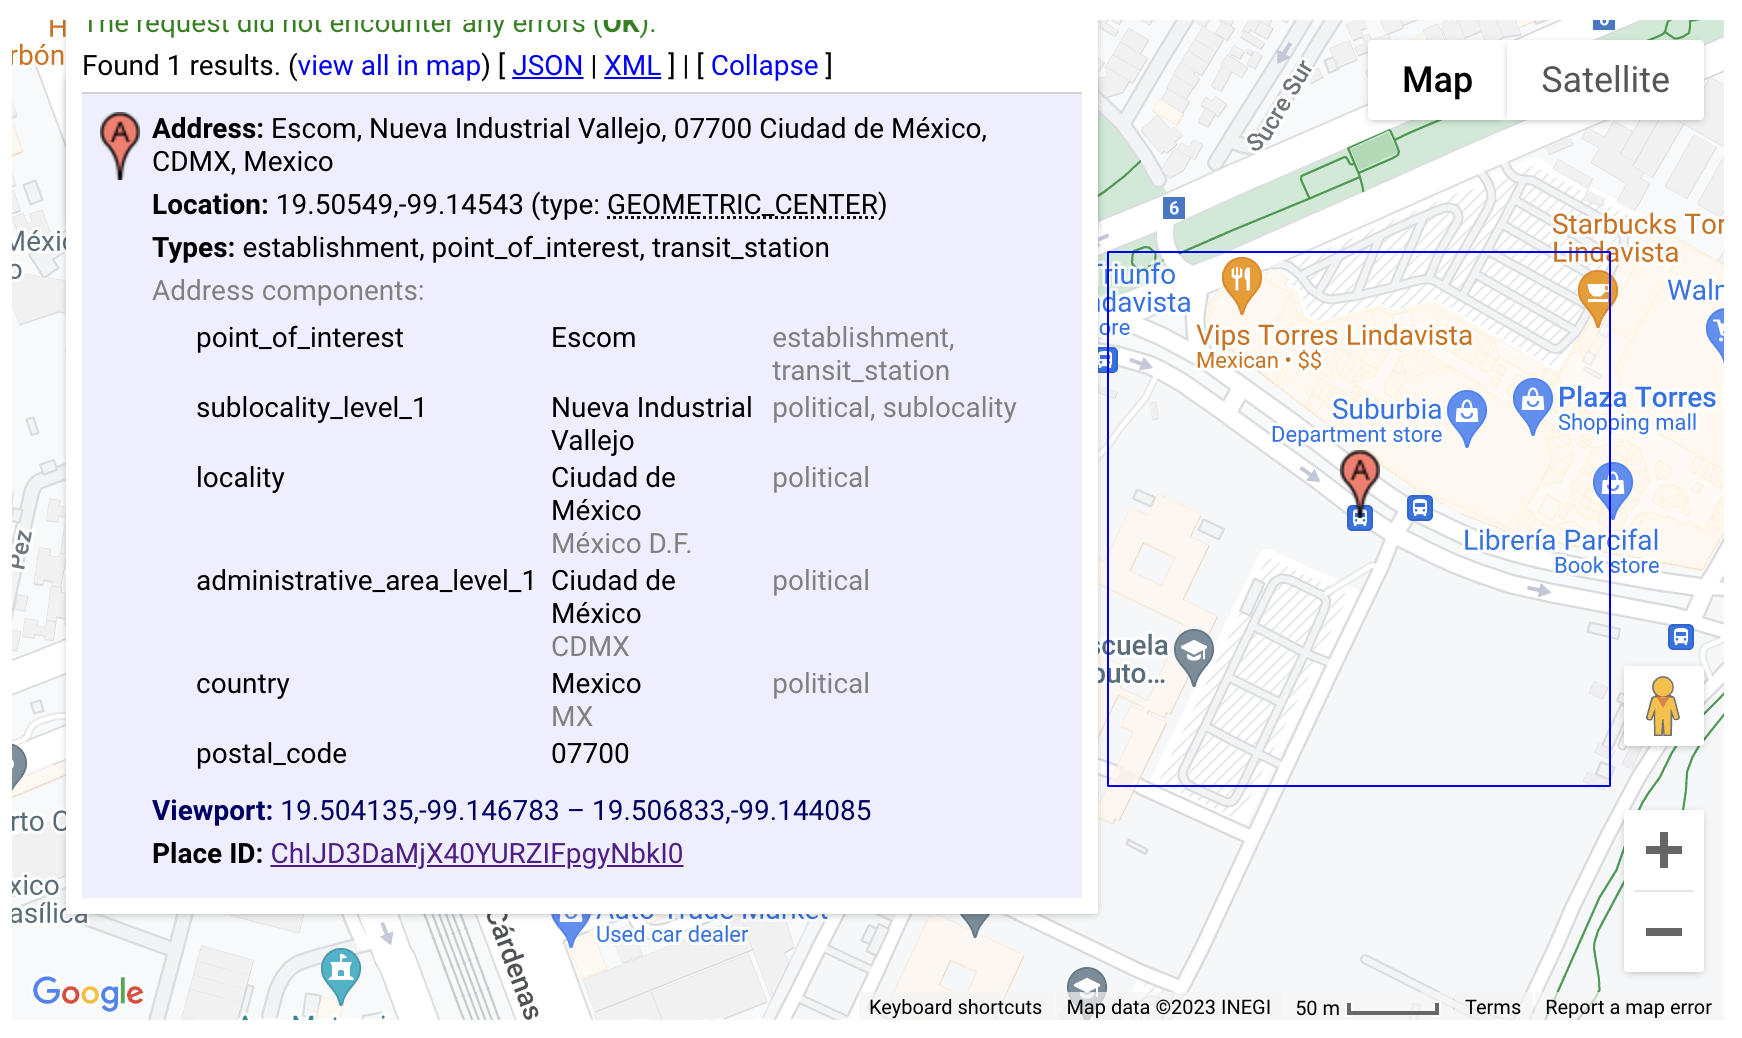
\includegraphics[width=0.8\textwidth]{imagenes/04-diseno/api-geocode-google-maps.png}
    \caption{Funcionalidad de geo-localización de Google Maps}
    \label{fig:google-maps}
\end{figure}


